% !TEX root = ../arbeit.tex
\chapter{Requirements}\label{chapter:requirements}
The build \ac{PROCAMS} is intended to be used by end users in order to investigate their behaviour with everywhere projections. The requirements for this \ac{PROCAMS} are deduced from the findings of the previously accomplished interviews. They are structured in a hardware and software section.

\section{Hardware}
First of all the \ac{PROCAMS} consists of two main components: a projector and a camera. The projector should be lightweight, light intensive and most important have an autofocus, which continuously focuses on the desired \emph{surface}. The camera is necessitate to interact with the \ac{PROCAMS}. To realise simple touch interaction a depth camera is reasonable \cite{Wilson:2010bv,Klompmaker:2012id}.
To achieve a \ac{PROCAMS} which can project to different \emph{interaction spaces} of the room, parts of the system need to be movable. At least the projector and the camera must be able to rotate in two \acl{DOF}. According to 50\% of the participants, alignment  should be possible without any manual effort.


Besides the projector and the camera, the system needs a computational unit which handles at least pre-processing of the camera images, video output to the projector and control of the movement of the unit. Furthermore, there needs to be a wireless link for data transmission as well as a loudspeaker and microphone for audio in- and output. These are the minimum hardware requirements to fulfil the majority of use-cases mentioned in the interviews. A first schematic sketch (see~\autoref{img:sketch}) illustrates how such a system could look like.

\begin{figure}[htbp] 
   \centering
   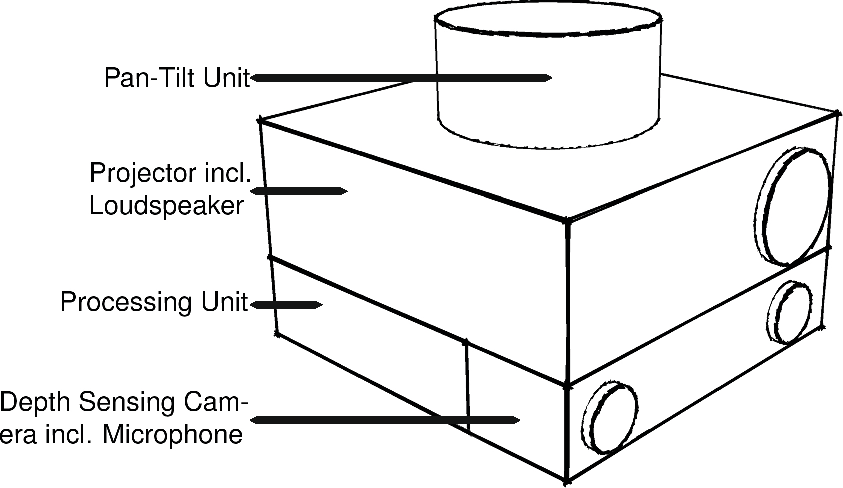
\includegraphics[width=\textwidth]{images/requirements/sketch_3.pdf} 
   \caption{Schematic sketch of a \ac{PROCAMS}}
   \label{img:sketch}
\end{figure}

\section{Software Framework}
The scope of operation of the hardware is very similar to many other systems \cite{Hardy:2012jo,Xiao:2013dp,Wilson:2012fb,Raskar:2005jy}. But for the user, an efficient working software is as important as a capable and light hardware. To enable frustration-free usability, the system must be usable with a minimum of configuration task. As far as possible configuration and calibration have to be done in the background hidden from the users perspective. For example, after creating a new \emph{interaction space} by aligning the system to the desired space the user should not have to calibrate the system or manually set the focus. All he has to do is to place the \emph{display} to the desired location.

The PROCAMS should be tilted and paned via remote to enable simple changes of the \emph{interaction space}. The space the projector is illuminating. Furthermore, it should be possible to store and load the current settings, including the actual alignment of the system, the position of \emph{displays} and therein rendered widgets. This means that the user is able to load previously stored settings and the \ac{PROCAMS} automatically aligns to this \emph{interaction space} and projects the last shown widgets to the stored positions. In addition, it should be possible to dynamically add and remove \emph{displays} to the \emph{surfaces} without the need to do manual adjustments for a rectified projection.

Development of widgets should be unproblematic and be deployed effortless into the framework in order to enable new rich content. Interaction with widgets should mainly be done via touch input. An alternative input method could be plain speech commands to trigger events like moving to a previously defined \emph{interaction space}. All in all the software framework should disburden the user from unnecessary tasks and allow intuitive use of user-friendly widgets.